\chapter{Implementación del software\label{sec:Implementacion_soft}}

Una vez finalizado el soporte físico del sistema, será necesario implementar a nivel de software todas las funciones deseadas.

El sistema está compuesto por tres microcontroladores, cada uno de ellos con sus propias características y métodos de programación. Debido a esto, a lo largo de este capítulo se explicará con detenimiento el software utilizado individualmente para ellos así como los distintos entornos de desarrollo (\acrshort{IDE}) necesarios.

Los distintos elementos se presentarán siguiendo el mismo orden que la información que se desea adquirir. Este es:
ADS $\Rightarrow$ Microcontrolador $\Rightarrow$ Interfaz inalámbrica $\Rightarrow$ PC.

\section{Microcontrolador STM32F4\label{Software_micro}}

Debido a la complejidad de los microcontroladores de la familia STM32, los desarrolladores han dedicado su tiempo y esfuerzo en crear herramientas que faciliten su programación. Estas herramientas llamadas \acrshort{IDE} contienen una recopilación de funciones, utilidades y ejemplos que simplifican sensiblemente el proceso de diseño e implementación del software que ejecutará el microcontrolador.

Es tan grande la comunidad de desarrolladores que hay detrás del STM que numerosas empresas han visto como una oportunidad de negocio la creación de un \acrshort{IDE} propietario.

\clearpage

\begin{figure} [h]
    \centering
    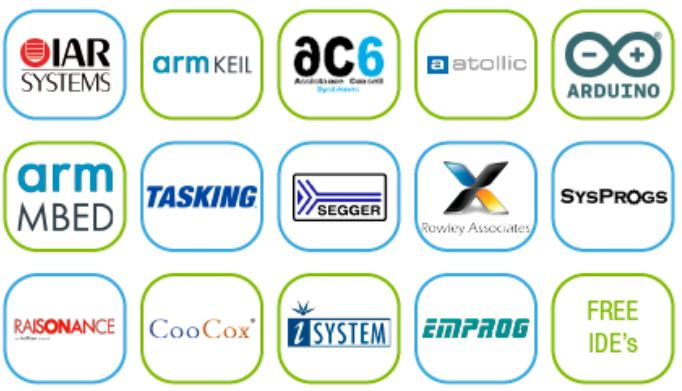
\includegraphics[width=13cm]{STM32_IDEs}
    \caption{IDE's alternativos disponibles \cite{STM32_IDEs}}
    \label{fig:STM32_IDEs}
\end{figure}

La figura \ref{fig:STM32_IDEs} muestra algunos entornos de desarrollo recomendados por el fabricante en su propia página web. Como se puede apreciar, en la imagen se hace distinción entre las opciones comerciales (azul) y las gratuitas (verde).


Software
	Comunicación ADS - STM
	
	Comunicación STM- ESP
	
	Arduino (Comunicación ESP - PC)
	
	